\section{Long Short Term Memory Modell}
Die erste \ac{LSTM}-Netzwerk Architektur wurde von \cite{Hochreiter1997} vorgestellt, um das Vanishing Gradient Problem zu lösen.\footcite[Vgl.][S. 5931]{VanHoudt2020} Dieses Problem tritt hauptsächlich bei einem \ac{RNN} auf.\footcite[Vgl.][]{Informatik2003}
\ac{LSTM}-Netzwerke sind also die Weiterentwicklung der klassischen \ac{RNN}-Netzwerke.\footcite[Vgl.][]{Hochreiter1997}
Heute bilden sie die Grundlage für sogenante Transformer, welche für Large Language Modelle benutzt werden.\footcite[Vgl.][]{Vaswani2017}


\subsection{LSTM Netzwerk Architektur}

Der Datenfluss einer LSTM-Zelle ist in Abbildung \ref{abb:lstm} dargestellt und lässt sich mathematisch durch folgende Gleichungen beschreiben:
\begin{align}
    f_t &= \sigma(W_f \cdot v_t + b_f) \label{eq:1a} \\
    i_t &= \sigma(W_i \cdot v_t + b_i) \label{eq:1b} \\
    \widetilde{C}_t &= \tanh(W_C \cdot v_t + b_C) \label{eq:1c} \\
    c_t &= f_t \ast c_{t-1} + i_t \ast \widetilde{C}_t \label{eq:1d} \\
    o_t &= \sigma(W_o \cdot v_t + b_o) \label{eq:1e} \\
    h_t &= o_t \ast \tanh(c_t) \label{eq:1f}
\end{align}
wobei $\sigma$ die Sigmoid-Funktion bezeichnet und $W_n$ klassische neuronale Netzwerke sind ($n = f, i, C, o$)\footcite[Vgl.][S. 5]{Chen2022}

\begin{figure}[htb]
    \centering
    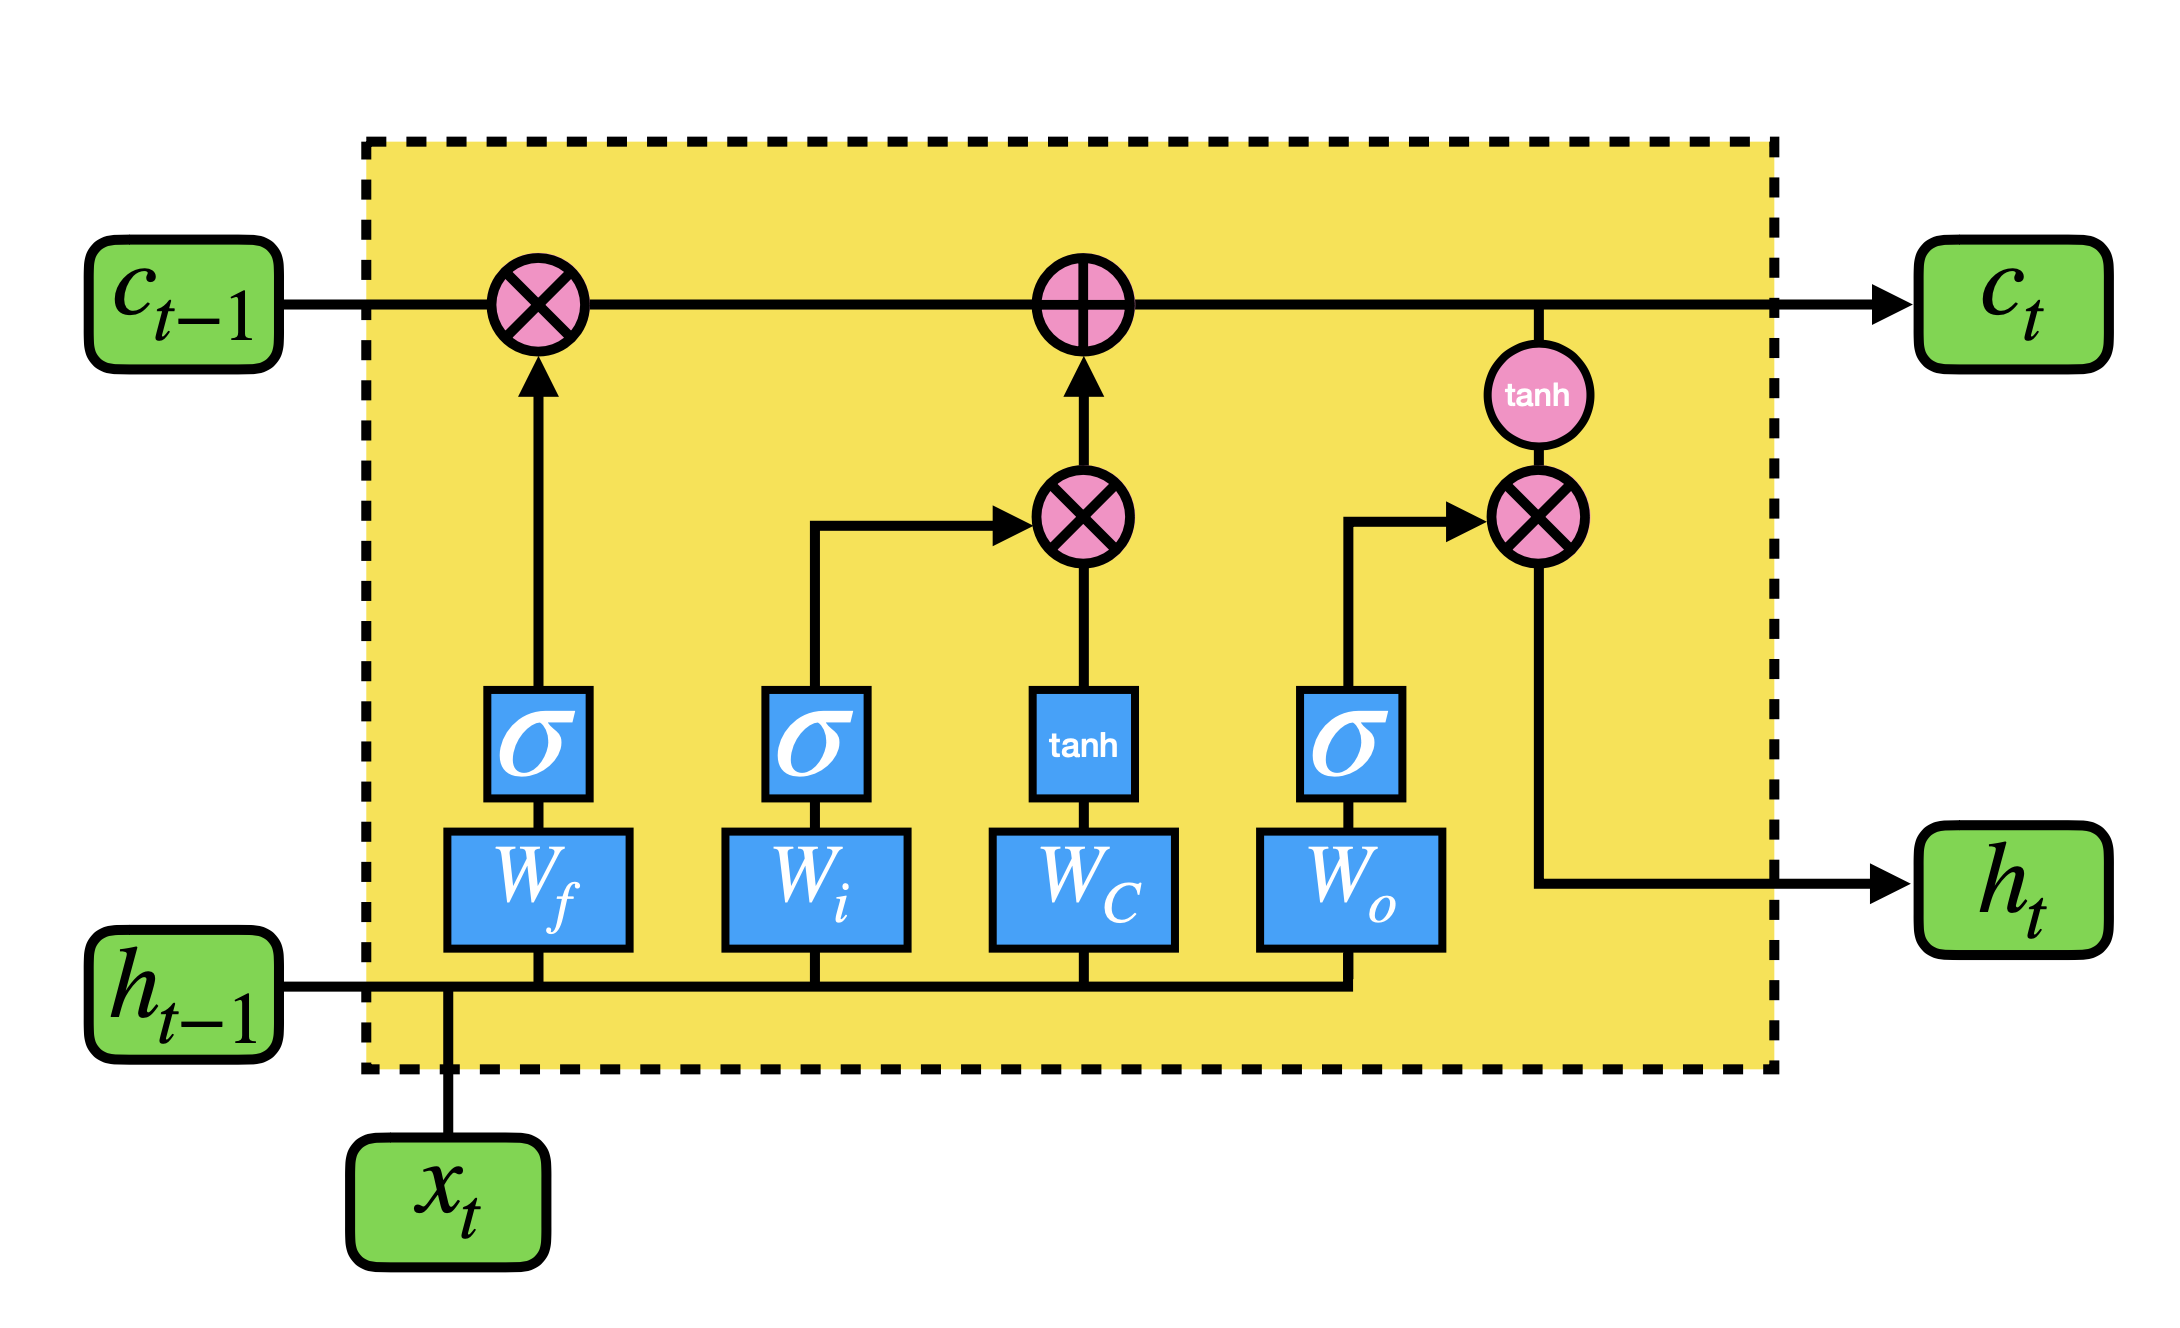
\includegraphics[width=13cm]{lib/graphics/LSTM.png}
    \caption[Long Short Term Memory Architektur]{\ac{LSTM} Zellen Architektur entnommen aus~\cite[S. 6]{Chen2022}}
    \label{abb:lstm}
\end{figure}

Die obenbeschriebenen Formeln und Zellenstruktur werden zum größten Teil genau so in der aktuell diskutierten Literatur verwendet.\footcite[Vgl.][]{Chen2022, Yu2023, Qi2021, Yan2018, Fischer2018, Liu2019, Sak2014, Sagheer2019}
In einigen Publikationen sind die Formlen leicht abgewandelt, da es auch andere \ac{LSTM}-Varianten gibt.\footcite[Vgl.][S. 5931f.]{VanHoudt2020} Das ändert die obenbeschriebene Grundstruktur allerdings nicht. Diese Struktur wird auch in der Literaturanalyse von \cite{VanHoudt2020} als klassische \ac{LSTM} bezeichnet.

Die klassische \ac{LSTM}-Architektur besteht aus drei Gates, welche die Eingabe $x_t$ verarbeiten (Input Gate), eine Ausgabe $h_t$ erzeugen (Output Gate) und den Zustand $c_t$ der Zelle verwalten (Forget Gate).\footcite[Vgl.][S. 5932]{VanHoudt2020}
Das Forget Gate ist in der ursprünglichen Version von~\cite{Hochreiter1997} nicht enthalten und wurde erst durch~\cite{Gers2000} hinzugefügt.
Durch diese drei Gates wird der Informationsfluss der \ac{LSTM}-Zelle geregelt und es ist möglich, dass die Zelle Informationen über beliebige Zeitintervalle hinweg speichern kann.\footcite[Vgl.][S. 5931]{VanHoudt2020}
Diese Informationen sind in den zwei Zuständen gespeichert, während $c_t$ der Langzeit-Speicher und $h_t$ der Kurzzeit-Speicher ist.\footcite[Vgl.][S. 5932f.]{VanHoudt2020}




Es ist möglich aus \ac{LSTM}-Architekturen mehrdimensionale Netzwerke zu konstruieren.\footcite[Vgl.][]{Sak2014}~\cite{Sagheer2019} beschreiben ein Deep \ac{LSTM}-Netzwerk, wobei mehrere \ac{LSTM}-Zellen hintereinander geschaltet werden.\footcite[Vgl.][S. 206]{Sagheer2019}
Deep \ac{LSTM}-Netzwerke werden in der Literatur beispielsweise für Finanzprognosen\footcite[Vgl.][]{Liu2019, Fischer2018, Yan2018} oder Bedarfsprognosen\footcite[Vgl.][]{Rodrigues2019} verwendet.

Für die in Kapitle \ref{design} aufgesetzt und durchgeführten Experimente, werden nur eindimensional Netzwerke betrachtet, da die in Kapitel~\ref{vergleichsobjekte} betrachteten \ac{QLSTM}-Architekturen alle auf eindimensionalen Netzwerken basieren.\footcite[Vgl.][]{Chen2022, Yu2023,Qi2021}
Auch andere in dieser Arbeit nicht analysierte \ac{QLSTM}-Modelle benutzten die zuvor genannten Formeln und Zellenstruktur.\footcite[Vgl.][]{Cao2023}



\subsection{Modell Training und Evaluation}\label{trainTest}

Bei Machine Learning Modellen ist es wichtig, dass nicht nur die Trainingsdaten korrekt vorhergesagt werden, sondern auch neuen, ungesehene Daten. Um diese Generalisierung des Modells zu erreichen, wird das Modell mit ungesehenen Testdaten evaluiert.\footcite[Vgl.][S. 191]{Panesar2021}
Wie der Datensatz in Trainings und Testdaten gesplittet wird ist Anwedungsfall abhängig.~\cite[][]{Chen2022} splitten den Datensatz beispielsweise bei $\frac{2}{3}$.

Die Initialisierung der Gewichtsmatrizen erfolgt in der Regel zufällig, wobei die Gewichte oft mit einer Normalverteilung initialisiert werden.\footcite[Vgl.][]{Chen2022, Sak2014}
\cite[][]{Sak2014} beispielsweise initialisiert die Gewichte mit einer Normalverteilung zwischen $[-0.2, 0.2]$.
Um diese zufällig instanziierten Gewichte, welche die verschiedenen \ac{LSTM}-Komponeten verbinden, zu trainieren, wird ein Optimierungsverfahren angewandt. Hierbei wird eine Verlustfunktion minimiert, die die Differenz zwischen den Vorhersagen und den tatsächlichen Werten berechnet.
Diese Verfahren basieren auf dem Konzept der Backpropagation erstmal vorgestellt durch~\cite{Werbos1990}. 
Das bedeutet, dass der Zellenzustand \(c(t)\) während der Backpropagation Gradienten von \(y(t)\) sowie vom nächsten Zellenzustand \(c(t+1)\) erhält.\footcite[Vgl.][S. 5933]{VanHoudt2020} Das führt dazu, dass die Gradienten akkumuliert werden, um alle Gewichtsmatrizen bestmöglich anzupassen. 
Basierend auf dieser Backpropagation gibt es verschiedene Optimierungsverfahren wie beispielsweise Stochastic Gradient Descent oder Adam\footcite[Vgl.][]{Kingma2014}.

Ist ein Modell trainiert, wird die Qualität der Vorhersagen bzw. die Generalisierung evaluiert.
Für die Evaluierung der Testergebnisse, stehen verschiedene Fehlermetriken zur Verfügung. LSTM Publikationen benutzten häufig den \ac{RMSE}/\ac{MSE}\footcite[Vgl.][]{Yu2023,Sagheer2019,Chen2022} und den \ac{MAE} \footcite[Vgl.][]{Chen2022}.
Welche Metriken am besten geeignet sind, hängt stark von der Modellarchitektur und -aufgabe ab.\footcite[Vgl.][S. 201]{Panesar2021}


Formeln der Evaluationsmetriken:
    \[ MAE = \frac{1}{n} \sum_{i=1}^{n} |y_i - \hat{y}_i| \]
  
    \[ MSE = \frac{1}{n} \sum_{i=1}^{n} (y_i - \hat{y}_i)^2 \]
  
    \[ RMSE = \sqrt{\frac{1}{n} \sum_{i=1}^{n} (y_i - \hat{y}_i)^2} \]
